\documentclass{standalone}
\usepackage{tikz}
\begin{document}
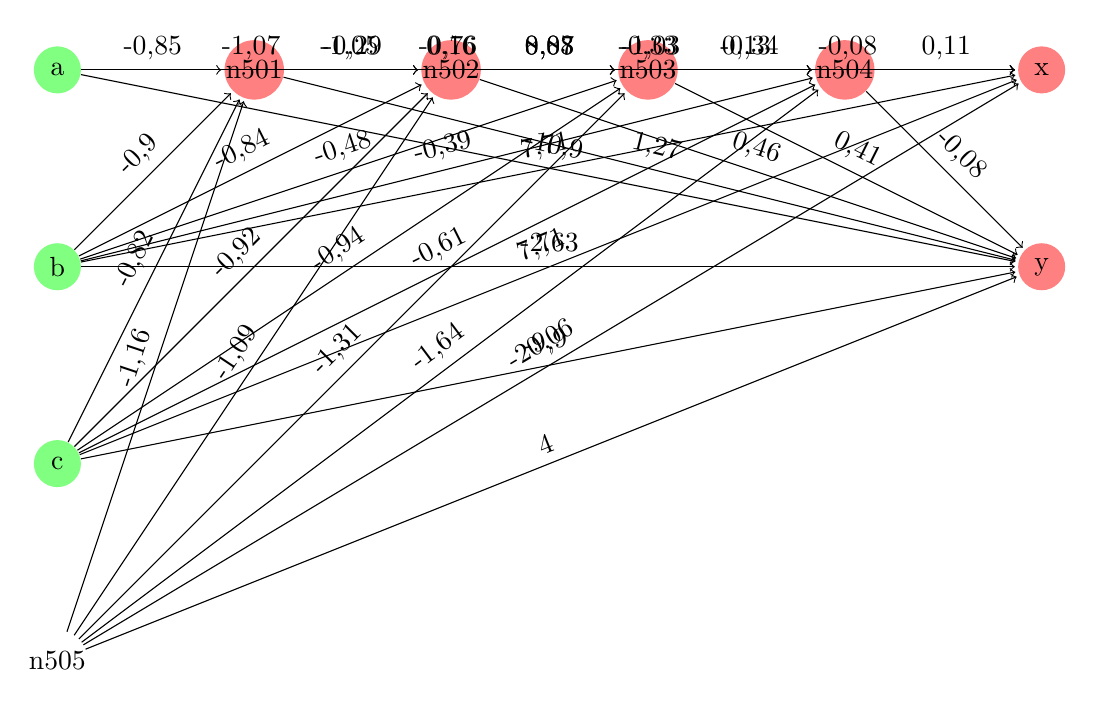
\begin{tikzpicture}[shorten >=1pt,->,draw=black!,node distance=2.5cm]
\tikzstyle{neuron}=[circle,fill=black!25,minimum size=17pt,inner sep=0pt]
\tikzstyle{constant}=[neuron, fill=white!50];
\tikzstyle{identity}=[neuron, fill=green!50];
\tikzstyle{sigmoid}=[neuron, fill=red!50];
\node [identity] (a) {a};
\node [identity,below of=a] (b) {b};
\node [identity,below of=b] (c) {c};
\node [constant,below of=c] (n505) {n505};
\node [sigmoid,right of=a] (n501) {n501};
\node [sigmoid,right of=n501] (n502) {n502};
\node [sigmoid,right of=n502] (n503) {n503};
\node [sigmoid,right of=n503] (n504) {n504};
\node [sigmoid,right of=n504] (x) {x};
\node [sigmoid,below of=x] (y) {y};
\path[every node/.style={sloped,anchor=south,auto=false}]
(n505) edge node {4} (y)
(n505) edge node {-1,16} (n501)
(n505) edge node {-20,06} (x)
(n505) edge node {-1,64} (n504)
(n505) edge node {-1,09} (n502)
(n505) edge node {-1,31} (n503)
(b) edge node {-2,63} (y)
(b) edge node {7,71} (x)
(b) edge node {-0,84} (n502)
(b) edge node {-0,9} (n501)
(b) edge node {-0,39} (n504)
(b) edge node {-0,48} (n503)
(a) edge node {8,83} (x)
(a) edge node {-0,76} (n504)
(a) edge node {-0,85} (n501)
(a) edge node {-10,9} (y)
(a) edge node {-1,05} (n503)
(a) edge node {-1,07} (n502)
(n502) edge node {0,46} (y)
(n502) edge node {-0,34} (x)
(n502) edge node {-0,33} (n504)
(n502) edge node {0,08} (n503)
(c) edge node {7,71} (x)
(c) edge node {-0,82} (n501)
(c) edge node {-9,9} (y)
(c) edge node {-0,94} (n503)
(c) edge node {-0,92} (n502)
(c) edge node {-0,61} (n504)
(n501) edge node {-1,03} (x)
(n501) edge node {1,27} (y)
(n501) edge node {0,16} (n503)
(n501) edge node {-0,29} (n502)
(n501) edge node {0,07} (n504)
(n504) edge node {-0,08} (y)
(n504) edge node {0,11} (x)
(n503) edge node {-0,08} (x)
(n503) edge node {0,41} (y)
(n503) edge node {0,13} (n504)
;\end{tikzpicture}
\end{document}